
%(BEGIN_QUESTION)
% Copyright 2010, Tony R. Kuphaldt, released under the Creative Commons Attribution License (v 1.0)
% This means you may do almost anything with this work of mine, so long as you give me proper credit

Suppose you need to measure the temperature of an operating oven using nothing but a 1000 $\Omega$ RTD ($\alpha$ = 0.00385), a 1.75 k$\Omega$ precision resistor, and a battery of unknown voltage:

$$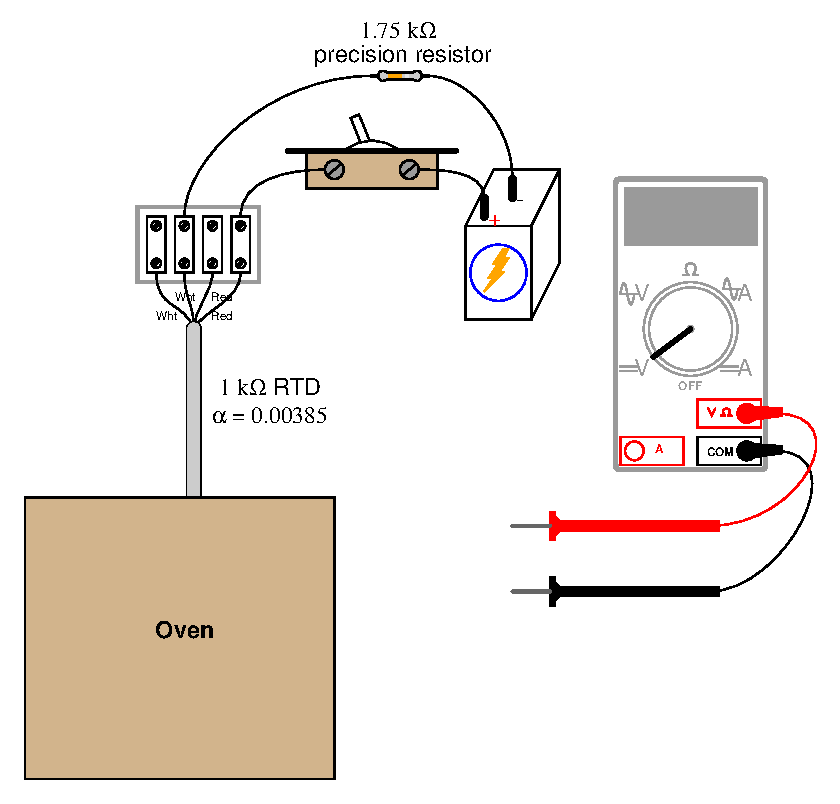
\includegraphics[width=15.5cm]{i00632x01.eps}$$

Turning the switch on, you measure 1.32 volts across the resistor and 1.22 volts across the RTD.  Calculate the oven temperature based on these measurements, and also explain why it is important to {\it quickly} take these measurements once the switch is turned on.

\underbar{file i00632}
%(END_QUESTION)





%(BEGIN_ANSWER)

$R_{RTD}$ = 1.617 k$\Omega$

\vskip 10pt

$T_{oven}$ = 160.4 $^{o}$C = 320.7 $^{o}$F (calculated from formula, not from a table)

\vskip 10pt

The voltage measurements must be taken very soon after the switch is thrown to avoid measurement errors due to ``self-heating'' of the RTD.

%(END_ANSWER)





%(BEGIN_NOTES)


%INDEX% Measurement, temperature: RTD 

%(END_NOTES)

